\chapter{System Build and Estimation}
\label{ch:estimate}

The specification in Chapter~\ref{ch:method} is not yet a plant. This chapter places it in an automation architecture and then estimates its behaviour by integrating the model of Section~\ref{sec:problem} over the week of Table~\ref{tab:regimes}. The architecture is buildable with equipment that a brewery treatment room already uses: a programmable controller for interlocks and inner loops, drives on the fans, a historian, and an edge computer for the minute-scale law and the soft sensor. The estimate is a simulation of that representative train. Absolute kilowatt-hours belong to the parameter set written in Chapter~\ref{ch:previous}. The comparisons belong to the information each controller is allowed to use.

\section{System build}
\label{sec:build}

\subsection{What is being built}

The build covers the cleaning plant from the inlet screen to the discharge flume. Production equipment upstream is not modified. The only production interface is a read of the batch and clean-in-place schedule. Figure~\ref{fig:train} is the process line the control system is drawn against. Liquid flows left to right. Air is a second network, drawn under the tanks that need it. The optimizer of Chapter~\ref{ch:method} writes set-points into this line. It does not replace the line.

\begin{figure}[ht]
\centering
\begin{tikzpicture}[
  font=\scriptsize,
  unit/.style={draw, rounded corners=2pt, minimum width=16mm, minimum height=9mm, align=center, inner sep=1pt},
  arr/.style={-{Stealth[length=2mm]}, thick}
]
\node[unit] (sc) {screen};
\node[unit, right=4mm of sc] (eq) {equalization};
\node[unit, right=4mm of eq] (ph) {pH};
\node[unit, right=4mm of ph] (an) {anaerobic};
\node[unit, right=4mm of an] (daf) {flotation};
\node[unit, right=4mm of daf, fill=blue!8] (ae) {aerobic};
\node[unit, right=4mm of ae] (cl) {clarifier};
\node[unit, right=4mm of cl] (out) {discharge};
\draw[arr] (sc) -- (eq);
\draw[arr] (eq) -- (ph);
\draw[arr] (ph) -- (an);
\draw[arr] (an) -- (daf);
\draw[arr] (daf) -- (ae);
\draw[arr] (ae) -- (cl);
\draw[arr] (cl) -- (out);
\node[unit, fill=orange!15, below=8mm of eq] (ex1) {exhaust\\fans};
\node[unit, fill=orange!15, below=8mm of daf] (ex2) {exhaust\\fan};
\node[unit, fill=orange!15, below=8mm of ae] (bl) {three\\blowers};
\draw[arr] (ex1) -- (eq);
\draw[arr] (ex2) -- (daf);
\draw[arr] (bl) -- (ae);
\end{tikzpicture}
\caption{Cleaning train. Shaded units are the fan duties. Anaerobic pretreatment is in the train so the aerobic fans see a polishing load rather than raw brewery waste.}
\label{fig:train}
\end{figure}

Levels of control follow the enterprise-control split \cite{isa95}. Level 0 is the drives, valves, and sensors. Level 1 is the programmable controller, programmed in the languages of IEC 61131-3, and it is the only level that may drop a run command or open a contactor \cite{iec61131}. Level 2 is the edge computer that runs Algorithm~\ref{alg:deployed} and the soft sensor. Level 3 is the historian and the schedule import. The optimizer is not Level 1. If the edge computer stops, Level 1 continues on the proportional-integral loop with the last legal set-point, and it is required to do so without a download. That fallback is the difference between an optimization project and an operable plant \cite{obrien2011,olsson2012ica,iratni2019}.

\begin{figure}[ht]
\centering
\begin{tikzpicture}[
  font=\small,
  layer/.style={draw, minimum width=11.2cm, minimum height=9mm, align=center, anchor=west},
  arr/.style={{Stealth[length=2mm]}-{Stealth[length=2mm]}, thick}
]
\node[layer, fill=yellow!15] (l3) at (0,0) {Level 3 \quad historian, schedule import, laboratory results};
\node[layer, fill=blue!10] (l2) at (0,-1.15) {Level 2 \quad edge computer: fan law and oxygen-transfer sensor};
\node[layer, fill=orange!12] (l1) at (0,-2.3) {Level 1 \quad programmable controller: interlocks and inner loops};
\node[layer, fill=green!10] (l0) at (0,-3.45) {Level 0 \quad drives, valves, probes, power meters};
\draw[arr] (0.2,-0.45) -- (0.2,-0.7);
\draw[arr] (0.2,-1.6) -- (0.2,-1.85);
\draw[arr] (0.2,-2.75) -- (0.2,-3.0);
\end{tikzpicture}
\caption{Control levels. Set-points move downward. Health bits and measurements move upward. Only Level 1 energizes a fan.}
\label{fig:levels}
\end{figure}

\subsection{Signals}

Table~\ref{tab:io} is the signal list the two technologies add to a plant that already has level, pH, and on--off control. It is not a full input-output schedule of the treatment works. It is the list without which Algorithm~\ref{alg:deployed} and the residual \eqref{eq:lphys} cannot be computed. Power meters are included on purpose. A fan law that trusts a commanded speed and never reads power cannot evaluate the middle residual of \eqref{eq:lphys}, and it cannot detect a machine that is on the schedule and off the shaft.

\begin{table}[ht]
\centering
\caption{Signals added for the fan optimizer and the transfer sensor. Scan times are Level~1 scan or faster. The edge computer subscribes at one-minute averages.}
\label{tab:io}
\begin{tabular}{@{}p{4.6cm}p{2.4cm}p{6.0cm}@{}}
\toprule
Signal & Direction & Use \\
\midrule
Delivered airflow, header & in & Inversion \eqref{eq:invert}, surge check, $K_La$ curve \\
Header pressure & in & Consistency with \eqref{eq:dp-num} \\
Blower power, each machine & in & Map residual, energy account \\
Blower speed, each machine & in & Surge law \eqref{eq:surge} \\
Blower run command & out & Staging word from Level 2, gated by Level 1 \\
Dissolved oxygen, aerobic & in & Bias \eqref{eq:bias}, balance residual \\
Temperature, aerobic & in & Saturation and $\theta$ correction \\
Influent flow and regime flag & in & Load scale $\sigma$, sensor window \\
Exhaust-fan speed, two rooms & out & Calendar fraction $\nu(\rho)$ in \eqref{eq:exhaust} \\
Schedule message & in & Preview $D$, detergent flag \\
Sensor health bit & internal & Fusion rule \eqref{eq:alpha-fuse} \\
\bottomrule
\end{tabular}
\end{table}

Communication from Level 1 to Level 2 is an OPC Unified Architecture session on the plant network, with the schedule message as a separate subscription from the production historian \cite{mahnke2009opc,isa95}. The edge computer does not sit on the drive network. A failure of the optimizer must not be a failure of the drive bus. Time synchronization is required only to a second. The lags in the plant are tenths of an hour. A one-second clock error is invisible next to the $0.75\,\mathrm{h}$ preview.

\subsection{Interlocks that override the optimizer}

The programmable controller enforces the following regardless of the set-point it has just received. A blower may not start if its outlet valve is shut. A blower that reports a drive fault is removed from the staging count and the edge computer is told the new $n_{\max}$. Header pressure above a mechanical trip stops all but one machine and opens a blow-off. Dissolved oxygen below \SI{0.4}{\milli\gram\per\litre} for more than ten minutes forces $n$ upward if a machine is available, even if the optimizer is silent. The exhaust fans run if their tank level is above the low-low cutout. None of these rules is an optimization. They are the reason Level 1 exists. The estimation below does not need to hit them on the nominal week. The build is incomplete if they are only in a manual.

Motor efficiency class is part of the build and not part of the control law. Machines on a variable-speed aeration duty should be specified to the current efficiency class for converter-fed motors, and the fan curve should be the tested curve, not a catalogue cube law \cite{iec60034,amca210,dixon2014turbo}. The power model \eqref{eq:polytropic} then uses the tested efficiency inside $\eta$. In the estimation, $\eta$ is the constant product $0.70\times 0.95\times 0.97$. A site curve would replace that product and would be read by the same residual.

\subsection{Software cycle}

The edge cycle is one minute, aligned to the historian. Inside the minute the sequence is fixed. Read averages. Update the $\alpha$ filter \eqref{eq:alpha-lag}. Evaluate the sensor residual on the last window and set the health bit. Run Algorithm~\ref{alg:deployed}. Publish $q$, $n$, and $\nu$. Log the residual, the health bit, the load scale, and the active degradation row of Table~\ref{tab:degrade}. Logging the degradation row is what makes a later audit possible. A plant that only logs dissolved oxygen cannot explain a week in which the calendar feed was down.

The proportional-integral fallback is tuned once, stored in the programmable controller, and not retuned by the edge computer. Its set-point is \SI{2.5}{\milli\gram\per\litre}, its proportional gain on airflow is $1400\,\mathrm{Nm^{3}\,h^{-1}}$ per $\mathrm{mg/L}$, and its integral gain is $500\,\mathrm{Nm^{3}\,h^{-1}}$ per $\mathrm{mg/L}$ per hour, with the integrator clamped at $\pm 8\,\mathrm{mg\,h\,L^{-1}}$ in the units of the implemented sum. Those are the gains of the baseline in Section~\ref{sec:est}, so the fallback the plant will actually run is the fallback the estimate measures. Gains that exist only in a paper and not in the controller image are not part of the build.

\subsection{Model used for the estimate}

The plant integrated in the estimate is exactly \eqref{eq:monod}--\eqref{eq:dp-num}, with the lags stated in Section~\ref{sec:problem}. The dissolved-oxygen update is semi-implicit,
\begin{equation}
\label{eq:semi}
C^{+}
=
\frac{
C
+
\Delta t\,
\big(
K_La\,\beta C^{*}
-
\mathrm{OUR}
\big)
}{
1
+
\Delta t\,
K_La
},
\end{equation}
which is the exact step of a linear transfer term and does not ring when $K_La$ is large. Substrate and ammonia use forward Euler with $\Delta t=0.02\,\mathrm{h}$. The controller is evaluated on the same grid and held between its own decisions. Four closed loops are integrated for $168\,\mathrm{h}$ from the same initial state ($S_{b}=40$, $S_{i}=30$, $S_{n}=4$, $C=2$, all in $\mathrm{mg/L}$).

The four loops are:

\begin{enumerate}[leftmargin=1.6em,itemsep=0.35em]
\item \textbf{Proposed.} Algorithm~\ref{alg:deployed}, lagged true $\alpha$ as the best case of the soft sensor, calendar preview of $0.75\,\mathrm{h}$, set-points \eqref{eq:dosp}.
\item \textbf{Proportional-integral.} The fallback gains above, fixed set-point \SI{2.5}{\milli\gram\per\litre}, no calendar, no $\alpha$.
\item \textbf{Fixed-$\alpha$ inversion.} Equation~\eqref{eq:invert} with $\alpha$ locked at $0.55$, load scale $\sigma=1$, set-point \SI{2.0}{\milli\gram\per\litre}, and the same bias filter. This is predictive control without either technology.
\item \textbf{Constant speed.} Airflow fixed at $1.15$ times the inversion of the fermentation clean-in-place equilibrium uptake at $\alpha=0.40$ and $C=\SI{2.2}{\milli\gram\per\litre}$, which evaluates to \SI{6552}{\nmcph}. The machine runs at that flow all week.
\end{enumerate}

Constant speed is the policy a plant uses when the drives are installed and nobody trusts a loop, or when the loop is in manual at the worst-hour valve position. It is the right first baseline. The proportional-integral loop is the right second baseline, because it is what Level 1 already contains. The fixed-$\alpha$ inversion separates the value of prediction from the value of $\alpha$ and the calendar.

The soft sensor in the proposed loop is not a freshly trained network with a random residual. It is the lagged true $\alpha$, filtered by \eqref{eq:alpha-lag}, with a two-percent caution. Chapter~\ref{ch:method} already called this an upper bound. The estimate therefore answers the question ``what is the information worth if the sensor is good,'' and not the question ``what residual will a particular training run leave.'' A commissioning test against off-gas is still required before the upper bound is treated as a site forecast \cite{leu2009,redmon1983}.

\section{Estimation}
\label{sec:est}

\subsection{Week totals}

Table~\ref{tab:week} gives the blower electricity and the discharge result for the four loops. Chemical oxygen demand violation hours count the time the aerobic effluent $S_{b}+S_{i}$ exceeds \SI{125}{\milli\gram\per\litre}. On this week, with this volume and this permit, every loop records zero violation hours. That fact is the first result and it should not be rounded into a claim of superior compliance. The tank and the kinetic ceiling can meet the study limit even when dissolved oxygen sags, provided the sag is not held for a long time near zero. The loops separate on energy and on how close they come to the dissolved-oxygen floor, not on a violation count that is zero for all of them.

\begin{table}[ht]
\centering
\caption{Blower electricity and discharge over the representative week. Violation hours are time above \SI{125}{\milli\gram\per\litre} chemical oxygen demand. The last column is energy divided by the constant-speed energy.}
\label{tab:week}
\small
\begin{tabular}{@{}lrrrr@{}}
\toprule
Loop & kWh & Mean kW & Viol.\ (h) & Fraction of constant speed \\
\midrule
Proposed & 9656 & 57.5 & 0 & 0.31 \\
Fixed-$\alpha$ inversion & 9620 & 57.3 & 0 & 0.31 \\
Proportional-integral & 10920 & 65.0 & 0 & 0.35 \\
Constant speed & 31151 & 185.4 & 0 & 1 \\
\bottomrule
\end{tabular}
\end{table}

Against constant speed, the proposed loop uses $31151-9656=21495\,\mathrm{kWh}$ less in the week, which is $69.0\%$. Against the proportional-integral fallback, it uses $10920-9656=1264\,\mathrm{kWh}$ less, which is $11.6\%$. Against the fixed-$\alpha$ inversion it uses $36\,\mathrm{kWh}$ more, about $0.4\%$. The last comparison is the interesting one. A predictive inversion that holds a sensible set-point already captures almost all of the energy. What the schedule and the live $\alpha$ buy on this week is not another large energy cut. They buy dissolved-oxygen margin during the detergent window, which the next table shows, and they buy a controller that does not depend on an operator having chosen \SI{2.0}{\milli\gram\per\litre} in advance. The proportional-integral loop holds \SI{2.5}{\milli\gram\per\litre} because that is the operator habit encoded in the fallback. The economic set-points \eqref{eq:dosp} are lower in the quiet hours and are the main reason the proposed loop beats the fallback on energy.

At an illustrative price of $0.12$ currency units per kilowatt-hour, used only as a conversion and not as a tariff study, the week is worth about $152$ currency units against the proportional-integral loop and about $2580$ currency units against constant speed. Over fifty-two such weeks the constant-speed gap is of order $1.3\times 10^{5}$ currency units a year on blower electricity alone. The number scales with the price and with how often the plant actually sits at the worst-hour valve. It does not scale the physics.

Flow over the week is
\begin{equation}
\begin{aligned}
&50\times 96
+
70\times 30
+
75\times 18
+
68\times 12
+
22\times 12
\\
&\quad
=
4800+2100+1350+816+264
=
9330\,\mathrm{m^{3}}.
\end{aligned}
\end{equation}
Specific blower energy of the proposed loop is $9656/9330=1.03\,\mathrm{kWh/m^{3}}$. The proportional-integral loop is $1.17\,\mathrm{kWh/m^{3}}$. Constant speed is $3.34\,\mathrm{kWh/m^{3}}$. Chemical oxygen demand mass fed to the aerobic tank is $3747\,\mathrm{kg}$ in the week, so the proposed loop uses $2.58\,\mathrm{kWh}$ per kilogram of aerobic influent chemical oxygen demand. These normalizations are arithmetic on Table~\ref{tab:regimes} and Table~\ref{tab:week}. They are the right way to carry the result to a plant with a different weekly volume, and they are not a license to ignore a different $\alpha$.

\begin{figure}[ht]
\centering
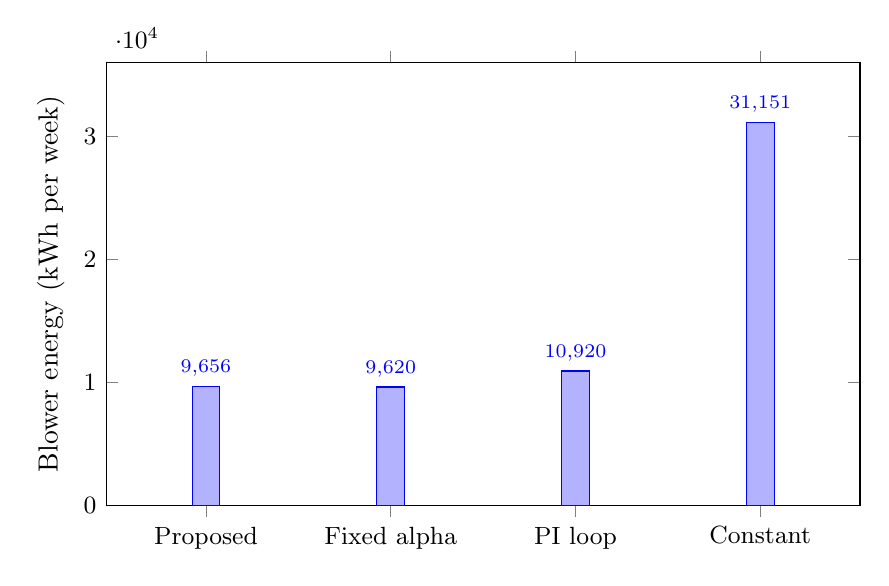
\begin{tikzpicture}
\begin{axis}[
  ybar,
  bar width=10pt,
  width=0.92\textwidth,
  height=7.2cm,
  ylabel={Blower energy (kWh per week)},
  symbolic x coords={Proposed, Fixed alpha, PI loop, Constant},
  xtick=data,
  ymin=0,
  ymax=36000,
  nodes near coords,
  every node near coord/.append style={font=\scriptsize, /pgf/number format/fixed},
  enlarge x limits=0.18,
  tick label style={font=\small}
]
\addplot coordinates {(Proposed,9656) (Fixed alpha,9620) (PI loop,10920) (Constant,31151)};
\end{axis}
\end{tikzpicture}
\caption{Blower electricity over the representative week. The large gap is between constant speed and any loop that moves the fans. The gap between the two predictive laws is not visible at this scale and is discussed with the dissolved-oxygen minima instead.}
\label{fig:energy-bars}
\end{figure}

\subsection{Where the energy is spent}

Table~\ref{tab:regenergy} splits blower energy and mean dissolved oxygen by regime. The proposed loop tracks \eqref{eq:dosp} in every production regime: mean dissolved oxygen is $1.81$, $2.02$, $2.18$, and $2.00\,\mathrm{mg/L}$ against set-points $1.8$, $2.0$, $2.2$, and $2.0$. On the weekend the set-point is $1.3$ but the mean is $4.46\,\mathrm{mg/L}$, because the mixing floor of \SI{900}{\nmcph} delivers more oxygen than the weekend uptake. The floor is doing what it was specified to do. Lowering it to save the weekend kilowatt-hours would put the single online machine on the surge side of \eqref{eq:surge}. The $247\,\mathrm{kWh}$ of the weekend is the price of that constraint, and it is already small next to the fermentation window.

\begin{table}[ht]
\centering
\caption{Blower energy and dissolved oxygen by regime for the proposed loop and the proportional-integral loop.}
\label{tab:regenergy}
\begin{tabular}{@{}lrrrrrr@{}}
\toprule
 & \multicolumn{3}{c}{Proposed} & \multicolumn{3}{c}{Proportional-integral} \\
\cmidrule(lr){2-4} \cmidrule(lr){5-7}
Regime & kWh & mean DO & min DO & kWh & mean DO & min DO \\
\midrule
Base, 96 h & 3469 & 1.81 & 1.72 & 4102 & 2.48 & 1.48 \\
Brewhouse, 30 h & 2438 & 2.02 & 1.39 & 2737 & 2.35 & 2.04 \\
Ferm.\ CIP, 18 h & 2441 & 2.18 & 1.63 & 2460 & 2.21 & 1.87 \\
Pack.\ CIP, 12 h & 1061 & 2.00 & 1.71 & 1318 & 2.61 & 2.33 \\
Weekend, 12 h & 247 & 4.46 & 0.86 & 304 & 5.17 & 2.78 \\
\bottomrule
\end{tabular}
\end{table}

The proportional-integral loop spends $4102-3469=633\,\mathrm{kWh}$ extra on the base regime alone, which is half of its weekly penalty. That is the cost of holding \SI{2.5}{\milli\gram\per\litre} for ninety-six hours when \SI{1.8}{\milli\gram\per\litre} already meets the discharge limit. During fermentation clean-in-place the two loops spend almost the same energy, $2441$ against $2460\,\mathrm{kWh}$, and they hold almost the same mean dissolved oxygen. The detergent window is not where this plant saves energy against a competent fallback. It is where a controller without the right $\alpha$ spends its margin, which is the fixed-$\alpha$ column of Table~\ref{tab:do-cip}.

Mean effluent chemical oxygen demand under the proposed loop is about \SI{56}{\milli\gram\per\litre} in base production, \SI{91}{\milli\gram\per\litre} in the brewhouse peak, \SI{94}{\milli\gram\per\litre} in fermentation clean-in-place, \SI{83}{\milli\gram\per\litre} in packaging clean-in-place, and \SI{39}{\milli\gram\per\litre} on the weekend. The hour-weighted mean is about \SI{67}{\milli\gram\per\litre}. All of these sit under the study limit, with the fermentation window the closest. The limit is not decorative. A longer detergent window, a lower $\alpha$, or a smaller tank would push that \SI{94}{\milli\gram\per\litre} up, and the hinge \eqref{eq:hinge-s} would then start to buy air the energy term does not want. On this week the hinge is inactive. The estimate should say so.

\begin{table}[ht]
\centering
\caption{Fermentation clean-in-place window, where $\alpha$ falls to $0.40$. Minimum dissolved oxygen is the quantity the live transfer estimate is for.}
\label{tab:do-cip}
\begin{tabular}{@{}lrrrr@{}}
\toprule
Loop & kWh in window & Mean DO & Min DO & Mean effluent COD \\
\midrule
Proposed & 2441 & 2.18 & 1.63 & 94 \\
Fixed-$\alpha$ inversion & 2186 & 1.88 & 0.90 & 96 \\
Proportional-integral & 2460 & 2.21 & 1.87 & 93 \\
Constant speed & 3339 & 2.92 & 2.90 & 90 \\
\bottomrule
\end{tabular}
\end{table}

Table~\ref{tab:do-cip} is the case for the second technology. The fixed-$\alpha$ inversion, which is otherwise as economical as the proposed loop, lets dissolved oxygen fall to \SI{0.90}{\milli\gram\per\litre} in the detergent window because it still believes $\alpha=0.55$. The proposed loop, reading $\alpha$ through the $0.30\,\mathrm{h}$ filter, bottoms at \SI{1.63}{\milli\gram\per\litre}. The energy cost of that margin is $2441-2186=255\,\mathrm{kWh}$ inside the window, and across the whole week the two loops differ by only $36\,\mathrm{kWh}$ because the proposed loop saves air in other hours by moving the set-point. A minimum of \SI{0.90}{\milli\gram\per\litre} is above the force-up interlock of \SI{0.4}{\milli\gram\per\litre} and below the operational floor of \SI{1.5}{\milli\gram\per\litre}. It is exactly the region in which nitrification slows, filamentous organisms are selected, and a plant can still post a legal chemical oxygen demand \cite{amand2013review,grady2011,rieger2014abac}. The soft sensor is justified on that floor, not on a kilowatt-hour race against an inversion that was already given a good set-point.

The proportional-integral minimum in the same window is \SI{1.87}{\milli\gram\per\litre}, which also clears the floor. Feedback can find the air if the integrator is allowed to move and the header has capacity. The price is the set-point it was given, paid mostly in the ninety-six quiet hours. The schedule-aware law clears the floor without that set-point. Constant speed clears the floor by a larger margin and pays \SI{3339}{\kilo\watt\hour} in a window where \SI{2441}{\kilo\watt\hour} is enough, and then keeps paying after the window has ended.

One minimum in Table~\ref{tab:regenergy} needs a plain reading. The proposed loop touches \SI{0.86}{\milli\gram\per\litre} on the weekend transition. The weekend mean is \SI{4.46}{\milli\gram\per\litre}, so the touch is a short transient as the load collapses and the bias \eqref{eq:bias} has not yet released the previous airflow command through the blower lag. It is a real defect of the deployed law at regime boundaries that cut the load, not a defect of the sensor. A practical correction, which the estimation did not turn on, is to allow $\sigma$ in \eqref{eq:scale} to fall below one when the previewed load is smaller, clipped for example at $0.7$. The upward clip at $1.35$ was written to avoid over-prediction. The missing downward clip is the weekend transient. It does not create a chemical-oxygen-demand violation on this week. It does cross the weekend floor of \SI{1.0}{\milli\gram\per\litre} briefly. The correction belongs in the next build of the edge image, and it is recorded here so the table is not tidied up after the fact.

\subsection{Exhaust fans and the combined fan account}

Equation~\eqref{eq:exhaust} at the regime speed fractions gives the exhaust-fan power: $6.33\,\mathrm{kW}$ in base production ($0.75^{3}\times 15\,\mathrm{kW}$), $9.21\,\mathrm{kW}$ in the brewhouse peak, $12.86\,\mathrm{kW}$ in both clean-in-place windows, and $2.49\,\mathrm{kW}$ on the weekend. The week is
\begin{equation}
\begin{aligned}
&6.33\times 96
+
9.21\times 30
+
12.86\times 18
+
12.86\times 12
+
2.49\times 12
\\
&\quad
=
608+276+232+154+30
=
1300\,\mathrm{kWh}.
\end{aligned}
\end{equation}
Added to the proposed blower total, the cleaning plant's fans use $9656+1300=10956\,\mathrm{kWh}$ in the week, of which the exhaust share is $12\%$. The exhaust schedule does not depend on which blower loop is selected. Reporting it separately keeps the $11.6\%$ and $69\%$ figures attached to the blowers, which are the machines the two technologies actually move. A combined percentage that mixed a fixed exhaust load into a blower saving would look smaller and would be worse arithmetic.

\subsection{Sensitivity the week already contains}

Three sensitivities are visible without a new plant model.

The mixing floor. Weekend blower energy is $247\,\mathrm{kWh}$ at a mean power of $20.6\,\mathrm{kW}$ even though the uptake would accept less air. Removing the floor would save that energy and would violate \eqref{eq:surge} for a single machine near \SI{2800}{\nmcph} rated flow. The floor stays.

The set-point habit. Moving the proportional-integral set-point from $2.5$ to the schedule \eqref{eq:dosp} would remove most of the $1264\,\mathrm{kWh}$ gap without a soft sensor. That experiment was not the baseline, because the fallback specified in Section~\ref{sec:build} is the habit, not the oracle. It is still the right operational remark: part of technology~1 is the set-point table, and it can be installed even if technology~2 is late.

The $\alpha$ error. Locking $\alpha$ at $0.55$ when the truth is $0.40$ is a relative error of $0.15/0.40=37.5\%$ on the transfer coefficient. The airflow inversion scales as $\alpha^{\,-1/0.82}$, so the missing air fraction before the bias integrator catches up is of order
\begin{equation}
\left(\frac{0.55}{0.40}\right)^{1/0.82}
-
1
=
1.375^{1.220}
-
1
\approx
0.47.
\end{equation}
A forty-seven percent air deficit, held for a fraction of an hour by the blower lag and the bias speed $K_{b}=0.55\,\mathrm{h^{-1}}$, is enough to mark the \SI{0.90}{\milli\gram\per\litre} minimum in Table~\ref{tab:do-cip}. The same arithmetic says what a worse detergent would do. At $\alpha=0.30$ the deficit factor becomes $(0.55/0.30)^{1.220}-1\approx 1.15$, and the header may hit $q_{\max}$ before the set-point is recovered. That case is outside the integrated week. It is the case in which the health bit and the table value in \eqref{eq:alpha-fuse} matter most, because the table for the fermentation recipe is $0.40$, already closer to the truth than the quiet-week $0.55$.

Calendar lead time. The preview of $0.75\,\mathrm{h}$ is several times the blower lag of $0.10\,\mathrm{h}$. Shortening it toward the lag would leave the minimum dissolved oxygen of the proposed loop closer to the fixed-$\alpha$ minimum. Lengthening it beyond the accuracy of the production clock would apply $\sigma>1$ too early and spend air the hinge does not require. The $0.75\,\mathrm{h}$ value is matched to the lags in the model. A site with a slower header should lengthen it, and should do so by measuring the header, not by copying the number.

\subsection{What the estimate does not show}

The integrator does not show a trained network's residual, a drifting diffuser $k_{0}$, a clarifier failure, an anaerobic upset beyond the influent table, a wrong recipe name, or a price that changes inside the week. It does not show three machines of unequal size, where the staging rule \eqref{eq:stage-rule} would be replaced by the integer program. It does not show a permit on suspended solids. It does not show that every brewery will save eleven percent against its existing loop. A plant that already runs ammonia-based aeration control at a low dissolved-oxygen set-point has less left to save against the proportional-integral column and still has the constant-speed column if any tank is in manual \cite{rieger2014abac,amand2012optimal,longo2016}.

Measurement uncertainty on the integrated comparison is the uncertainty of the parameters in \eqref{eq:kla-est} and \eqref{eq:dp-num}, not a Monte Carlo band around a stochastic influent. Those parameters were chosen so the quiet week and the detergent week are both oxygen-feasible. A diffuser whose clean-water $k_{\mathrm{ref}}$ is far below $6.5\,\mathrm{h^{-1}}$ would change the absolute power and could make the fermentation window infeasible at $n=3$. The acceptance test in commissioning is the hand inversion of Section~\ref{sec:saempc} against a measured header, plus one off-gas traverse on a detergent day \cite{asce2007oxygen,leu2009,gillot2005}. If the hand inversion and the meter disagree, the table in this chapter is not a forecast for that header.

Within those limits the estimate supports four sentences. Any of the three modulating loops cuts blower energy by about two thirds relative to constant speed sized for the detergent hour. The schedule-aware set-points cut about twelve percent relative to a competent proportional-integral loop parked at \SI{2.5}{\milli\gram\per\litre}, with no increase in hours above the study chemical-oxygen-demand limit. A predictive inversion without a live $\alpha$ matches that energy and gives up dissolved-oxygen floor during the detergent window, down to \SI{0.90}{\milli\gram\per\litre} against \SI{1.63}{\milli\gram\per\litre}. Exhaust fans add about \SI{1300}{\kilo\watt\hour} in the week under a calendar speed fraction and are not where the saving is. Those four sentences are the quantitative claim of the thesis.

\subsection{Implementation order}

A plant that accepted the specification would not install both technologies on the same day. The order implied by the estimate is the order of the tables. First, move constant-speed tanks onto the Level~1 proportional-integral fallback and confirm the interlocks. That step takes the large share of the energy and does not require an edge computer. Second, install the set-point table \eqref{eq:dosp} and the calendar subscription, still with $\alpha$ from the regime table rather than from the network. Table~\ref{tab:week} says this is where the remaining energy is. Third, train and commission the soft sensor against off-gas on a detergent day, and only then close \eqref{eq:alpha-fuse}. The third step is what protects the dissolved-oxygen floor when the detergent is worse than the table. Building them in the reverse order would put a network in the loop before the plant has a fallback worth falling back to.

The software image of the edge computer should be small enough to review: the inversion, the staging rule, the bias clamp, the health bit, and the log. The full horizon integer program can replace the staging rule when the machines stop being identical, and it should be validated against the rule on the identical-machine case before it is allowed to start a fan the rule would leave off. That validation is a regression test on recorded weeks, not a new theory. The theory this plant needs was already in the aeration-control and predictive-control literature cited in Chapter~\ref{ch:previous}. The part that was not in that literature is the use of the brewery calendar as the disturbance and the use of a transfer residual as the way $\alpha$ enters the fan command. The week integrated here is the estimate of what those two uses are worth when the sensor is good and the calendar is right.
